\documentclass{standalone}
\usepackage{tikz}
\usetikzlibrary{shapes,fit}

\begin{document}
\begin{tikzpicture}[
    scale=0.55,
    >=latex,
    line join=bevel,
    LN/.style={draw=gray!80!black,rectangle,line width=0.1em,minimum size=1.7em},
    BN/.style={draw=gray!80!black,circle,line width=0.1em,minimum size=1em,inner sep=1pt},
    CN/.style={draw=gray,line width=0.1em,densely dashed,rectangle,rounded corners,fill opacity=0.3},
    LL/.style={->,draw=gray!80!black,line width=0.1em}
  ]
  \node[LN] (l1) at (-150bp,0bp) {$\ell_1$};
  \node[LN] (l2) at (-50bp,0bp) {$\ell_2$};
  \node[LN] (l3) at (85bp,0bp) {$\ell_3$};
  \node[BN] (b1) at (-200bp,-75bp) {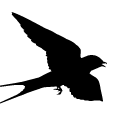
\includegraphics[width=0.5cm,trim=0 20 0 20,clip]{swallow.png}};
  \node[BN] (b2) at (-150bp,-75bp) {
\includegraphics[width=0.5cm,trim=0 20 0 20,clip]{hawk.png}};
  \node[BN] (b3) at (-100bp,-75bp) {
\includegraphics[width=0.5cm,trim=0 20 0 20,clip]{dove.png}};
  \node[BN] (b4) at (-50bp,-75bp) {
\includegraphics[width=0.5cm,trim=0 20 0 20,clip]{crow.png}};
  \node[BN] (b5) at (0bp,-75bp) {
\includegraphics[width=0.5cm,trim=0 20 0 20,clip]{thrush.png}};
  \node[BN] (b6) at (60bp,-75bp) {
\includegraphics[width=0.5cm,trim=0 20 0 20,clip]{duck.png}};
  \node[BN] (b7) at (110bp,-75bp) {
\includegraphics[width=0.5cm,trim=0 20 0 20,clip]{shorebird.png}};
  
  \node[CN,fill=magenta!50!black,fit=(b1)(b2)(b3)(b4)] (fit1) {};
  \node[CN,fill=lime!70!black,yscale=1.5,fit=(b3)(b4)(b5)] (fit2) {};
  \node[CN,fill=cyan!80!black,fit=(b6)(b7)] (fit3) {};
  
  \draw[LL] (l1) -- (-150bp,-48bp);
  \draw[LL] (l2) -- (fit2);
  \draw[LL] (l3) -- (fit3);
\end{tikzpicture}
\end{document}
